%=========================================
% 	   Fallbeispiel     		 =
%=========================================
\chapter{Fallbeispiel}
In diesem Kapitel stellen wir, eine anhand eines selbst ausgedachten Anwendungsfalls, eine Cloud-Native Architektur vor, die wir prototypisch implementiert haben.

\section{Beschreibung}
In unserem Beispiel haben wir einen Nachrichtendienst (ChatApp) entworfen. Benutzer können sich registieren, anmelden und Nachrichten an andere Benutzer senden. 


\section{Anforderungen}
\subsection{Nichtfunktionale Anforderungen}
1. Skalierbarkeit
Das System muss mit einer großen Zahl von Benutzern, die das System gleichzeit verwenden, umgehen können.

2. Verfügbarkeit
Das System muss zu jeder Zeit verfügbar sein.

3. Sicherheit
Das System muss Berechtigungen überprüfen können (z.B. darf Benutzer X die Nachrichten lesen) und das System sollte sich gegen übliche Cyberangriffe (z.B. DDoS) schützen können.

4. Änderbarkeit/Erweiterbarkeit
Das System muss so entworfen werden, dass weitere Komponenten (z.B. Hochladen von Bildern und Videos) einfach hinzugefügt werden können.

\subsection{Funktionale Anforderungen}
1. Registierung
Ein Benutzer kann sich mit seiner E-Mail Adresse und einem Passwort im System registieren.

2. Ein- und Ausloggen
Ein Benutzer kann sich mit seiner E-Mail Adresse und seinem Passwort im System anmelden und dann die Funkionen nutzen bis er sich abmeldet.

3. Nachrichten schreiben/lesen
Ein Benutzer kann Nachrichten an andere Benutzer senden und Nachrichten, die an ihn gesendet worden sind, abrufen.


\begin{figure}[bth] 
	\centering
	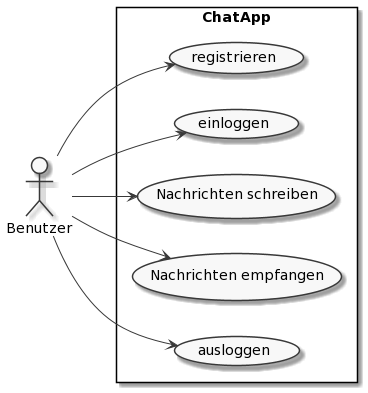
\includegraphics[width=0.6\textwidth]{Graphics/Usecase-Diagramm.png}
	\caption{Use-Case Diagramm}
\end{figure}

\section{Architekturentwurf}

\begin{figure}[bth] 
	\centering
	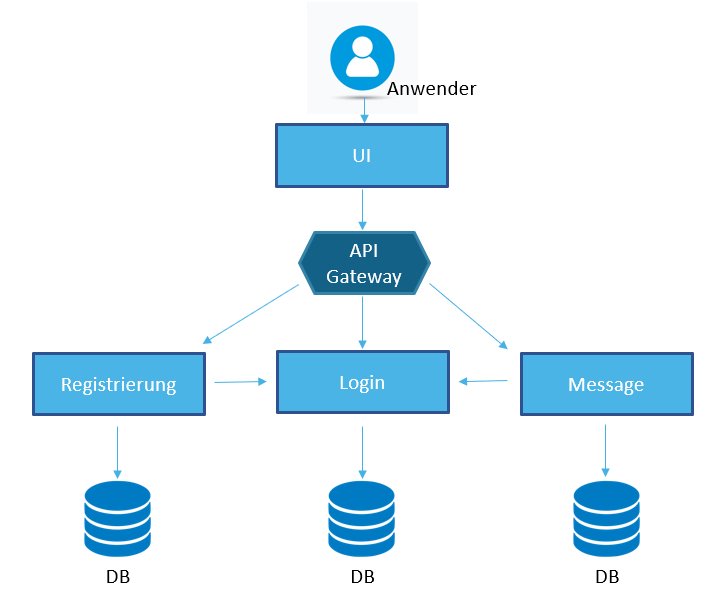
\includegraphics[width=0.6\textwidth]{Graphics/Architekturentwurf.png}
	\caption{Architekturentwurf}
\end{figure}

\begin{figure}[bth] 
	\centering
	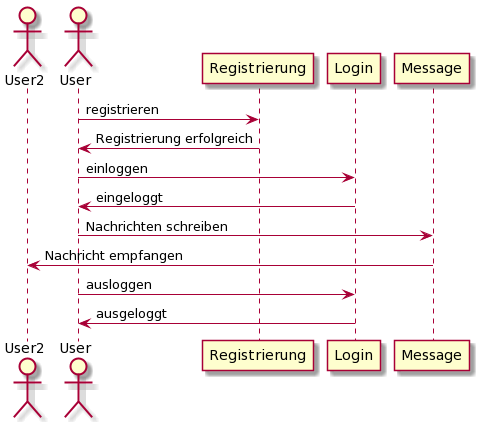
\includegraphics[width=0.6\textwidth]{Graphics/Sequenzdiagramm.png}
	\caption{Sequenzdiagramm}
\end{figure}

\section{Implementierung des Prototyps}
auch genutzte Technologien aufzeigen

